\chapter{Accommodation in Multiparty Interaction with An Agent}
\label{chap:speech_variations_in_hhci}

\lettrine{M}{ore} dynamic vocal behaviors can be established in interaction with more than two speakers.
This is not only due to additional possible connections between interlocutors, but also because of additional factors that might influence them as well, like the order of speech or the role of each speaker.
A \acl{hhci} study is presented in this chapter, where the effects of different aspects and conditions on vocal accommodation are investigated.

\pagebreak

\section{Speech variations in human-human-computer interaction}
\label{sec:accommodation_in_multiparty_interaction_with_an_agent}

Nowadays, we are witnessing an ever-growing presence of devices with spoken interaction capabilities in our everyday lives.
As argued in \cref{subsec:personal_assistants}, the use of \acp{pa} is rapidly increasing, as more mundane tasks can be achieved using them.
The question arises, therefore, whether different speech patterns and characteristics emerge in such \ac{hci} compared to \ac{hhi}; and if yes, which.
%One way of measuring these differences is in terms of linguistic similarity between the interlocutors.
%It has been demonstrated that humans may change their speech behavior when interacting with computer-based systems.
%In various \ac{hci} experiments, participants have been found to speak differently to computers and change their speech during the interaction \citep[e.g.,][]{Branigan2010linguistic}.
The vast majority of experimental work done in the field of vocal accommodation deals with the smallest social interactions, namely dyadic conversations.
Those can be dyads of two human speakers in \ac{hhi}, or a human and some computer-based agent in \ac{hci}.
Vocal accommodation in these types of interactions is explored in \cref{chap:shadowing_in_sung_music_and_human_computer_interaction,chap:conv_analysis}.
However, social interactions may also consist of three or more participants.
This is true for both \ac{hhi} and \ac{hci}, but also for interactions with mixed human and computer-based interlocutors and specifically multiple humans talking with a single device.
The latter can occur in various situations, like a person consulting a \ac{va} regarding availability in a weekly schedule while setting an appointment with a colleague or two friends ordering tickets from a voice-activated machine.
Mixed multiparty interactions already take place in various real-world situations lives.
Their popularity -- and sometimes necessity -- increase alongside the rise in use of \ac{c-ai} devices, such as \acp{va}, voice-activated cars, hands-free medical assistants, \acp{its}, social robots, and others.
It is important, therefore, to understand whether convergence, divergence, and other effects (like those described in \cref{subsec:variation_types}) may occur not only in \acp{hci}, but in \acfp{hhci} as well.
Various \ac{hci} experiments have shown that participants speak differently to computers and change their speech behavior during the interaction \citep[e.g.,][]{Branigan2010linguistic}.
Some works also compared the reaction of participants to different configurations of the computer-based interlocutor \citep[e.g.,][]{Levitan2016implementing}.
Yet, none of those has performed a comparison between human-directed and computer-directed speech within a single multiparty interaction.
Moreover, only the influence of the system's speech output on the user speech is typically examined in accommodation experiments, but not the influence of another human interlocutor.

Empirical work on multiparty \ac{hci} includes experiment where participants interact with different types of agents, like social robots \citep{Foster2012two, Ibrahim2019fundamental} and human avatars in immersive virtual worlds \citep{Traum2002embodied}.
Even in dyadic form, spoken interactions are a hard task for computers.
All the more so, when more than one other interlocutors are involved.
Measuring accommodation becomes more complex with multiple interlocutors involved, as discussed in \citet{Rahimi2019acoustic}.
There are many technical challenges on the way to realistic, real-time interactions with computers, including -- but not limited to -- center-of-attention detection, active speaker detection, turn taking, understanding private and shared knowledge, and of course correct speech production and understanding.
Interactions with machines are challenging for humans, too, since the former do not behave and react the same way (and often speed) as humans.
An example of such a social activity that is reasonably easy for humans to learn but still far from being feasible by computers are social games with a large number of participants.
These games typically require the players to be deceptive, track and exploit the behaviors of others, and react quickly to ever-changing dynamics between the players.
\Citet{Jonel2018Farmi} describe the challenges of such scenarios and discusses way to cope with them.
The type and severity of those problems depend also on the type of the computer-based agent (see \cref{sec:types_of_sdss}).
For instance, embodied agents at least have some basic way to convey non-verbal information, whereas voice-only systems like \acp{va} do not.
On the one hand, this gives a wider range of expressions to embodied systems, but requires more communication channels to implement and coordinate on the other hand.

This chapter presents a study that examines interaction-level vocal accommodation in \ac{hhci}.
In this paradigm, two human speakers work collaboratively with an agent to complete tasks while only one of them can talk directly to the agent.
More details about the dataset and the tasks are given in \cref{sec:vacc}.
Investigating such a scenario contributes to the understanding of both the role of an agent in interactions with multiple humans and the influence of another human in a \ac{hhci}.
These two aspects are examined in the two \emph{components} of the study:
The \emph{addressee} component focuses on the differences between the participant's addressed interlocutor within a conversation \citep[][see]{Raveh2019ESSV}, and the \emph{crowd} component spotlights the influence of an additional human interlocutor on the participant's speech toward the agent \citep[see][]{Raveh2019InterspeechAlexa}.
The question tackled by the second component is whether and to what extent speaking to a second human interlocutor in the same interaction as the agent influences the accommodation toward it, i.e., whether users speak differently towards a \ac{va} when another human participates in the interaction.
to that end, the distributional and temporal analyses performed in \cref{sec:analysis_hhci} are based on the participants' \emph{speech directions}, i.e., \acf{hds} and \acf{dds}, as illustrated in \cref{fig:condition_comparison_addressee,fig:condition_comparison_crowd}.

\section[The \acl{vacc}]{Dataset}
\label{sec:vacc}

\begin{figure}[t]
	\centering
	\subfigure[Solo condition]
	{\raisebox{1.85cm}{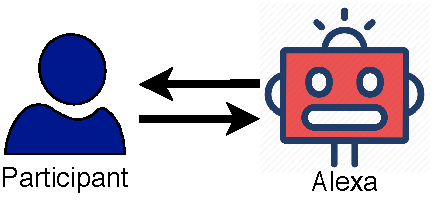
\includegraphics[width=0.45\textwidth]{condition_solo}}
	\label{fig:condition_solo}}
	\hfill
	\subfigure[Confederate condition]
	{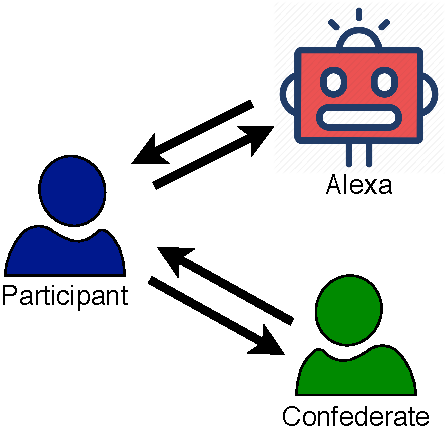
\includegraphics[width=0.45\textwidth]{condition_confederate}
	\label{fig:condition_confederate}}
	\caption[Solo and confederate conditions in \acs{hhci} setting]
		{Illustration of solo and confederate conditions.
		A black arrow represents direction of speech from speaker to addressee.
		Note that the confederate (in green) never talks or addressed by Alexa, but only the participant (blue).}
	\label{fig:conditions_comparison}
\end{figure}
%
The accommodations study presented here uses the \acf{vacc}\footnote{\url{http://www.iikt.ovgu.de/iesk/en/Research+Groups/MDS/Research/VACC-p-4624.html}}, introduced by \citet{Siegert2018VACC}.
This corpus is suitable for this study, because it comprises both \acp{hci} and \acp{hhci} with a 2\textsuperscript{nd} generation Amazon Echo Dot device using the default skill set and German female voice of the \acf{va} Alexa.
These configurations are referred to here as \emph{solo} and \emph{confederate} conditions, respectively.
\Cref{fig:conditions_comparison} illustrates the interlocutor relations in each condition.
Similar corpora were used to study automatic addressee detection \citep[e.g.,][]{Shriberg2013addressee, vanTurnhout2005identifying}.
Although the study here does not set addressee detection or classification as a goal, it aims to provide insights and accommodation-related measures that may be useful for such tasks.
In the \ac{vacc}, the male confederate was present in the room only during tasks in the confederate condition and always sat at the same location.
To simulate the spatial situation of a multi-party interaction with a \ac{va}, the participant and the confederate sat in similar distance from the device that was situated on a table, roughly forming an equilateral triangle \citep[see Figure 2 in][]{Siegert2018VACC}.
The participant had led the interactions with both the confederate and Alexa, and the confederate never talked to Alexa directly.
Therefore, in the confederate condition, the participant needed to alternately speak with the confederate and Alexa alternately as part of the same interaction, without explicitly signaling to whom each utterance is addressed.
%Two high-quality neckband microphones (Sennheiser HSP 2-EW-3) were used to capture the voices of the participant and the confederate speaker.
%Additionally a high-quality shotgun microphone (Sennheiser ME 66) captured the overall acoustics and the output of Amazon's Alexa.
Two tasks were performed in each condition:
In the calendar task, the participant's goal was to find available time slots for several hypothetical appointments with the confederate.
The participant's pre-defined calendar was stored on the device and was accessible only via inquiries to Alexa.
In the solo condition, the participants got written information about the confederate's availability, whereas in the confederate condition, the confederate could be asked about it.
The goal of the quiz task is to answer trivia questions, like \enquote{When was Albert Einstein born?}.
Since Alexa was not always able to immediately provide a full answer to all the questions, the required information could be gathered incrementally over multiple turns.
Here, the participant solved the quiz alone in the solo condition or teamed up with the confederate so that the two could discuss the question-asking strategy in the confederate conditions.
The calendar task was designed so that the way to its solution is relatively straightforward:
Query the device for possible times till a match is found.
This requires interacting mostly -- if not only -- with the computer-based interlocutor.
Indeed, this task typically elicited interactions, in which the participant interacted with the confederate or the device in discretely separate turn blocks in the confederate conditions.
\Ac{dds} blocks were, unsurprisingly, longer, as the confederate was only addressed when additional information about the task was required.
The quiz task's flow was more flexible, since the strategy as to which questions to ask Alexa can be determined by the participant, including the amount and frequency of the confederate's intervention in the confederate conditions.
Indeed, more dynamic alternations between \ac{hds} and \ac{dds} were observed in this task.
As a whole, the quiz task is less formal than the calendar task.

The dataset contains recordings of 27 (14 female) German native speakers in the age range of 20 to 32 years (mean 24~$\pm$3.3).
Each participant performed the quiz and calendar tasks in both solo and confederate conditions, for a total of 108 interactions (2 tasks $\times$ 2 conditions $\times$ 27 participants).
%An interaction was finished either by completing the task or by stopping it prematurely in case no further progress could be made, to avoid participant frustration.
%The latter, however, happened only a few times.
These interactions consist of approximately \num{13500} utterances, which were manually transcribed and annotated (speaker, speech times, addressee, etc.) and stretch over total recording time of \SI{17}{\hour} \SI{7}{\minute} (\SI{31}{\minute} average interaction length).
The permutations of the tasks, conditions, and their order were balanced.

%\begin{figure}[!h]
%	\begin{center}
%		\fbox{\parbox{6cm}{
%		This is a figure with a caption.}}
%		\includegraphics[scale=0.5]{image1.eps} 
%		\includegraphics[width=0.75\linewidth]{figures/IMG_4798.jpg}
%		\caption{A snapshot of the data collection setup. The confederate speaker (left side) and the participant (right side) are sitting around a table, where the voice assistant (Amazon Alexa Echo Dot) is located.}
%		\label{fig:wohnzimmer}
%	\end{center}
%\end{figure}


%The recordings were stored in WAV format with \SI{44.1}{\kilo\hertz} sample rate and 16 bit resolution.
%The recordings were manually separated into utterances, which were additionally annotated with its speaker, context, and textual transcription.
%The speaker of each utterance could be the participant, Alexa, or the confederate.
%The context marked the type of interaction of the utterance, which include \ac{hds}, \ac{dds}, cross-talk, off-talk, laughter, and more.
%To deal with clearer data, only \ac{hds} and \ac{dds} contexts were used for analysis in this paper.
%The transcription was obtained using the Google Cloud Speech API automatic speech recognition service.
%\cref{tab:dataset_charact} summarizes the dataset characteristics.

%\begin{table}[t]
%	% \captionsetup{format=plain,justification=raggedleft,width=.4\textwidth,hangindent=0pt,skip=500pt}
%	\centering
%	\caption{\ac{vacc} dataset characteristics}
%	\label{tab:dataset_charact}
%	\begin{tabular}{L{3cm}L{3cm}}
%		\toprule
%	     Participants 				& 27														\\
%	     Sex 						& Male 13 / Female 14 										\\
%	     Total Recorded Data 		& \SI{17}{\hour} \SI{7}{\minute}							\\
%	     Experiment Duration 		& Mean: 31 min 												\\
%		  Age (years)				& Mean 24 (Std: 3.32)										\\	% Min: 20; Max: 32  \\
%	     Language 					& German													\\
%	     Annotation 				& Transcription, Addressee, Laughter, Cross-Talk, Off-Talk	\\ 
%	     Supplementary self-reports & Evaluation of interaction, AttrakDiff, Speaking style, Experiences in interacting with voice assistants\\
%		\bottomrule
%	\end{tabular}
%\end{table}

\subsection{Annotations}
\label{subsec:annotations_hhci}

Each utterance in an interaction was annotated with its speaker, context, and textual transcription.
The speaker of each utterance could be the participant, Alexa, or the confederate.
Cross-talk was rare, as the participants typically waited till the confederate or Alexa finished talking (except for when they tried to interrupt Alexa mid-utterance if the response was unquestionably wrong or irrelevant due to recognition error).
The context marks the utterance's interaction type, like \ac{hds}, \ac{dds}, cross-talk, off-talk, laughter, and more.
To deal with clearer data, only \ac{hds} and \ac{dds} contexts were used for analysis, which, together, constituted over \SI{90}{\percent} of the interactions' recording time.
Transcriptions were obtained using the Google Cloud Speech API automatic speech recognition service and were subsequently manually verified and corrected.
Utterances' start and end times were derived directly from the transcriptions' timestamps.

\section{Analysis}
\label{sec:analysis_hhci}

\begin{figure}[t]
	\centering
	\subfigure[\acs{hds} in confederate condition]
	{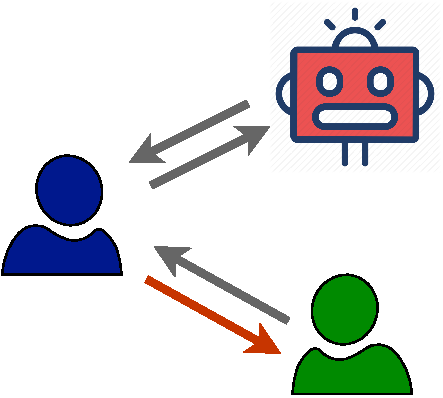
\includegraphics[width=0.45\textwidth]{condition_confederate_marked_hhi}
	\label{fig:condition_confederate_marked_hhi}}
	\hfill
	\subfigure[\acs{dds} in confederate condition]
	{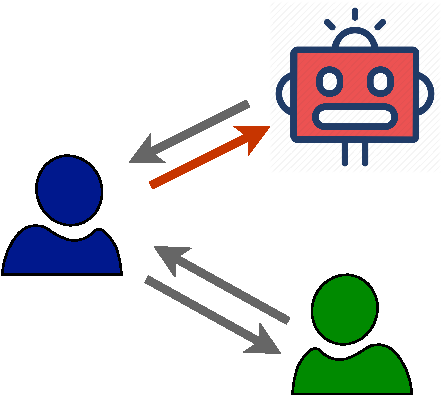
\includegraphics[width=0.45\textwidth]{condition_confederate_marked_hci}
	\label{fig:condition_confederate_marked_hci}}
	\caption[\acs{hds} and \acs{dds} compared in confederate condition]
		{Illustration of the compared speech directions in the \emph{addressee component}.
		The orange arrows mark the compared speech directions (participant to confederate and participant to Alexa).}
	\label{fig:condition_comparison_addressee}
\end{figure}

\begin{figure}[t]
	\centering
	\subfigure[\acs{dds} in solo condition]
	{\raisebox{1.6cm}{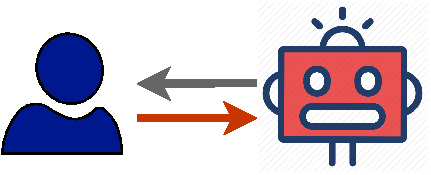
\includegraphics[width=0.45\textwidth]{condition_solo_marked}}
	\label{fig:condition_solo_marked}}
	\hfill
	\subfigure[\acs{dds} in confederate condition]
	{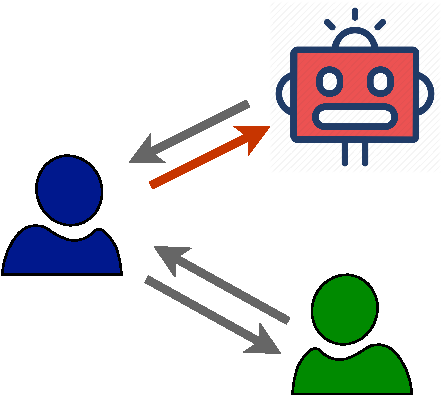
\includegraphics[width=0.45\textwidth]{condition_confederate_marked_hci}
	\label{fig:condition_confederate_marked_hci_crowd}}
	\caption[\acs{dds} compared in solo and confederate conditions]
		{Illustration of the compared speech directions in the \emph{crowd component}.
		The orange arrows mark the compared speech directions (participant to Alexa with and without the presence of the confederate).}
	\label{fig:condition_comparison_crowd}
\end{figure}

A subset of the \ac{vacc} was used for the analysis in each component, which is suitable for the speech directions in question.
\Cref{fig:condition_comparison_addressee,fig:condition_comparison_crowd} illustrate the examined speech directions in each component.
Only the 54 interactions from the confederate conditions were used for the addressee component, as the alternations between \ac{hds} and \ac{dds} within an interaction were examined.
For the crowd component, all 108 interactions were taken, because the comparison required executions of the tasks performed in both solo and confederate conditions.
Interactions of all 27 participants were included in both subsets.
Despite the different sizes of the subsets, the number of comparisons was the same for both components, since the addressee component used both speech directions of the participants in each interaction (54 $\times$ 2 = 108) and the crowd component used only \ac{dds} but from both conditions (54 $\times$ 1 + 54 $\times$ 1 = 108).
These subsets were analyzed based on the audio signals and the annotations described in \cref{subsec:annotations_hhci}.
The speaker annotations were used to determine to which of the three speakers the measured values should be ascribed.
The text transcriptions were only used for verifying the correct audio segments were analyzed.
Comparisons were made between the utterances of the same interaction, i.e., within a single task.

To increase temporal resolution, the audio signals were cut into two-seconds \emph{slices}.
A single slice always contained audio from a turn of a single speaker.
Any remainder shorter than 2 seconds got a separate slice.
For example, a turn of length \SI{5.2}{\second} was sliced into three slices of \SI{2}{\second}, \SI{2}{\second}, and \SI{1.2}{\second}.
This way, values measured in a slice could belong only to one speaker.
Splitting the turns also creates equal, consecutive, and more comparable time units for an interaction without introducing artificial boundaries by dividing it into a pre-defined number of parts \citep[as in][]{Silber-Varod2018prosodic}.
This is especially important for the temporal analysis (\cref{subsec:temporal_analysis}).
Slice lengths of 0.5, 1, 5, and 10 seconds were experimented with as well.
However, those were proved too short to capture changes in \ac{ar} (see below), which is dependent on the size of this window, or two long for a comparable and uniform temporal resolution.
Two seconds was found to be a good compromise based on these criteria.

The following phonetic features were targeted: 
%
\begin{description}%[wide=0pt, leftmargin=0.5\parindent, nosep]
	\item[\Acf{f0}] -- mean pitch measured within a slice with hop size of \SI{100}{\milli\second} and a pre-defined range of \SIrange{60}{350}{\hertz}.
	\citet{Gregory1993Voice} found that this feature is used to produce social similitude and cohesiveness in dyadic interviews.
	Moreover, this feature showed convergence effects in an auditory naming task \citep{Babel2012role} and a \ac{hci} shadowing task \citep{Bulatov2009effect}.
	
	\item[Intensity] -- mean intensity measured within a slice with hop size of \SI{100}{\milli\second}.
	This feature showed significant entrainment effects in game scenarios \citep{Levitan2011measuring} and as a indicator for social desirability \citep{Natale1975convergence}.
	
	\item[\Acf{ar}] -- the ratio of number of syllables to phonation time within a slice, as described in \citet{DeJong2009arcitulcationrate}.
	\citet{Schweitzer2013convergence} examined this feature in the context of phonetic convergence, but no effect was found on turn-level and interaction-level analyses.
\end{description}
%
All features were measured individually in each slice automatically using Praat \citep{Boersma2018praat} scripts.
The preprocessing and analysis were performed using the system introduced in \citet[][and see \cref{chap:web-based_responsive_spoken_dialogue_system}]{Raveh2018Specom}.

\section{Results}
\label{sec:results_hhci}

Two analyses were carried out: distributional and temporal.
The first looks at global differences on the interaction level of the participants' productions.
The second examines time-based, continuous changes in the similarity between the participants and the other interlocutors.

\subsection{Distributional analysis}
\label{subsec:distributional_analysis}

\begin{table}[b]
	\centering
	\caption[Percentage of significantly different interaction pairs in crowd component]
		{Percentages of interactions in which the distributional difference of each feature was significant}
	\label{tab:results_hhci_addressee}
	\begin{tabularx}{\linewidth}{XSSS}
		\toprule
		& \acs{f0} 						& {intensity}				& \acs{ar}									\\
		signif. diff.					& \SI{74}{\percent}			& \SI{89}{\percent}		& \SI{13}{\percent} \\
		\acs{hds} mean (\acs{sd}) 		& 10.5\,\si{\hertz}			& 2.95\,\si{\decibel}	& 0.627				\\
		\acs{dds} mean (\acs{sd}) 		& 10 \,\si{\hertz}		& 2.61\,\si{\decibel}	& 0.634				\\
		\bottomrule	
	\end{tabularx}
\end{table}
%
The means, medians, and \aclp{sd} of the target features in the participants' speech in each of the interactions were calculated for both \ac{hds} and \ac{dds}.
These measures shed light on the overall range of values used when the participant was talking to each of the other two interlocutors.
They were listed for each target feature chronologically throughout the interaction.
These lists were divided into four speech directions based on speaker and context:
the participant talking to the confederate, the participant talking to Alexa, the confederate talking to the participant, and Alexa talking to the participant (see four arrows in \cref{fig:condition_confederate}).
The contrast between \ac{hds} and \ac{dds} is observable within the participant's speech only, which was active in both contexts.
To detect these differences, the distribution of their respective values in the solo and confederate conditions in each interaction pair were compared.
This was done by using the two-sample Wilcoxon test \citep{Wilcoxon1945individual}, with $\alpha = 0.05$ with the null hypothesis that similar distributions of the target feature were used in both conditions.
A significant result of the test means that the participant produced the respective feature differently when interacting with Alexa alone compared to when the confederate participated as well.
\cref{tab:results_hhci_addressee} shows the percentage of interaction pairs, in which the null hypothesis was rejected, i.e., that the feature was utilized differently by the participant in each condition.

\begin{figure}
	\centering
	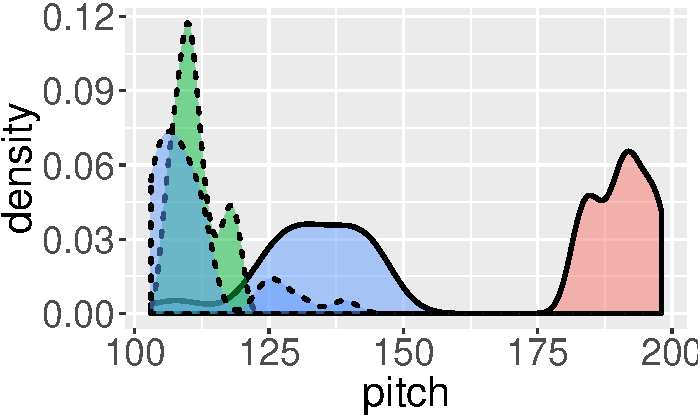
\includegraphics[width=.9\linewidth]{20171127A_Quiz_01_pitch_dist_cut}
	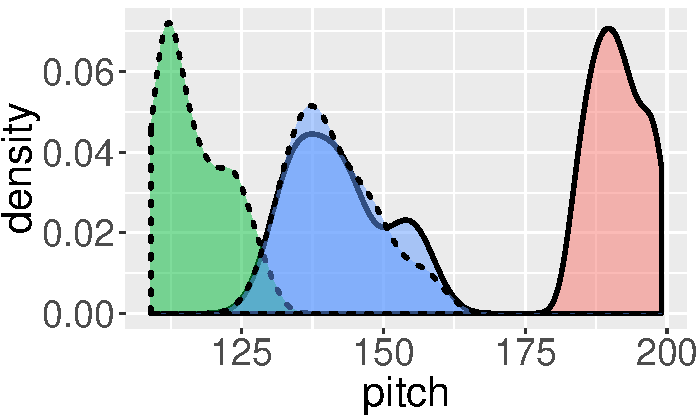
\includegraphics[width=.9\linewidth]{20171127C_Calendar_02_pitch_dist_cut}
	\vspace{0.3cm}
	\caption[Interactions with significant and insignificant \acs{f0} distributions difference between \acs{hds} and \acs{dds}]
		{Examples of \ac{f0} distributions in \ac{hds} and \ac{dds} with a \emph{significant} difference (top; quiz task of participant 20171127A; p~$\ll$~0.0001,~$\alpha=0.05$) and \emph{insignificant} difference (bottom; calendar task of participant 20171127C; p~=~0.71,~$\alpha=0.05$).
		The colors represent distributions of the  participant (blue), Alexa (red), and the confederate (green).
		The line style differentiates between \ac{hds} (dashed line) and \ac{dds} (solid line).}
	\label{fig:hds_dds_dist}
\end{figure}
%
\begin{figure}
	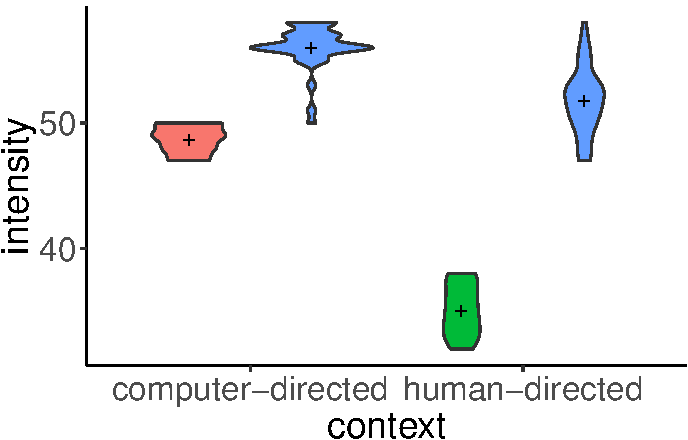
\includegraphics[width=.85\linewidth]{20171127A_Quiz_01_intensity_violin_cut}
	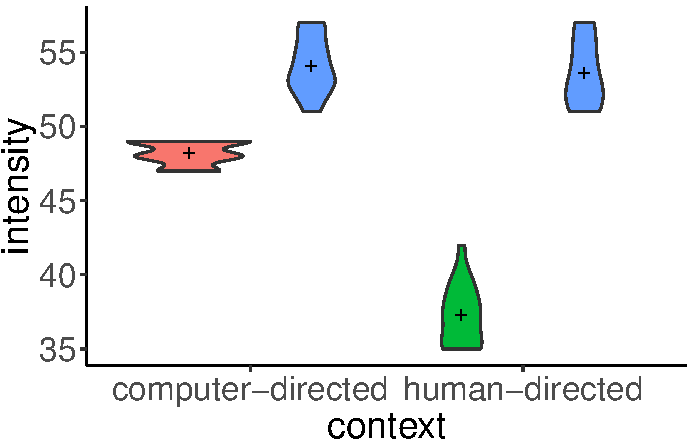
\includegraphics[width=.85\linewidth]{20171127C_Calendar_02_intensity_violin_cut}
	\caption[Interactions with significant and insignificant intensity distributions difference between \acs{hds} and \acs{dds}]
		{Examples of intensity distributions in \ac{hds} and \ac{dds} with a \emph{significant} difference (top; quiz task of participant 20171127A; p~$\ll$~0.0001, $\alpha=0.05$) and \emph{insignificant} difference (bottom; calendar task of participant 20171127C; p~=~0.55, $\alpha=0.05$).
		The colors represent distributions of the participant (blue), Alexa (red), and the confederate (green).
		The widths of a boxes represent the value frequencies and the \enquote*{+} sign marks their respective means.}
	\label{fig:hds_dds_violin}
\end{figure}

\Cref{fig:hds_dds_dist} show examples of the distributions of a participant's \ac{f0} in \ac{hds} and \ac{dds} contexts in the addressee component.
Since a female voice was always used for Alexa and the confederate was always male, there is a natural gap between their \ac{f0} values.
This gap leaves room for convergence to occur, i.e., change in the participants' production in the direction one of the other interlocutors.
As \cref{tab:results_hhci_addressee} shows, in \SI{74}{\percent} of the cases out of the 54 analyzed interactions the difference of the participant's \ac{f0} between \ac{hds} and \ac{dds} was significant.
Out of those, in \SI{85}{\percent} of the cases the distribution mass of \ac{dds} contained higher values than \ac{hds}'s, which indicates accommodation towards Alexa.
Unlike \ac{f0}, absolute intensity values may not be as meaningful due to the device's and the confederate's location relative to the participant's microphone.
This means that the absolute values of the participant's intensity in \ac{hds} and \ac{dds} can be compared directly, but only relatively against Alexa's and the confederate's.
Therefore, the differences of this feature as shown in \cref{fig:hds_dds_violin} should only be compared between the participant's both speech direction within an interaction.
These differences between the participants' \ac{hds} and \ac{dds} were significant in \SI{89}{\percent} of the cases.
In general, participants tended to speak to Alexa with a louder voice than to the confederate, although their distance from the participants was the same.
The differences between \ac{ar} distributions in \ac{hds} and \ac{dds} were significant in \SI{13}{\percent} of the cases.
This shows that the participants largely spoke with the confederate at the same speed as with Alexa.
Interestingly, the \ac{ar} was temporarily considerably lower when the participants tried to improve intelligibility, especially if the system's output indicated that it did not correctly understood the participant's utterance due to a recognition error.
%
\begin{table}
	\centering
	\caption[Percentage of significantly different interaction pairs in the addressee component]
		{Percentage of interaction pairs with significant differences with respect to each target feature with all the interactions together and separated by order tasks.}
	\label{tab:signif_conditions}
	\sisetup{table-format=3.0}
	\begin{tabularx}{\linewidth}{XSSS}
		\toprule
		\thead[l]{feature} & {\thead{any order}} & {\thead{solo first}}	& {\thead{confederate first}}\\
		\midrule
		\acs{f0}	& 67	& 72	& 60 \\
		intensity 	& 67	& 76	& 56 \\
		\acs{ar}	& 30	& 31	& 28 \\
		\bottomrule	
	\end{tabularx}
\end{table}
%
In the confederate component, the performed each task both alone and with the confederate.
Since chronologically, by design, one of the conditions needed to precede the other, the percentages were also calculated separately for the cases where tasks were performed first in the solo condition and then in the confederate condition, and vice versa.
This separation shows whether interacting first with Alexa alone, without any human input, influenced the vocal behavior of the participants.
As there were no breaks between the components, the only factors for change were the order of the conditions and the involvement of another human speaker.
As shown in \cref{tab:signif_conditions}, the percentages of significant differences when interacting first only with Alexa were indeed higher by \SI{12}{\percent}, \SI{20}{\percent}, and \SI{3}{\percent} for \ac{f0}, intensity, and \ac{ar}, respectively.
\cref{fig:signif_cases_ordered} further breaks down the differences between interaction pairs and introduces the factor of the performed task.
In line with the tendency shown in \cref{tab:results_hhci_addressee}, the features \ac{f0} and intensity have the highest percentages of significant cases, regardless of the performed task, and the tasks performed first show higher percentages of different distributions.
In the lower percentages, it is the task, rather than the target feature, that shows differences between the cases.
And last, for \ac{ar}, with the lowest percentages, there is a clear difference between the quiz and the calendar tasks.
All in all, the \texttt{task} factor was a good indicator only for the feature with the lowest difference percentage and the \texttt{order} factor was more informative for the features with higher percentages.
To sum up, these results show significant differences in the majority of the cases for two of the three features for both the addressee and crowd components.
These outcomes provide a look into further aspects of \ac{hds} and \ac{dds} and speech-related features in \ac{hhci}, which may help studies in topics like addressee detection or vocal accommodation in  multiparty interactions.
%
%
\begin{figure}[t]
	\centering
	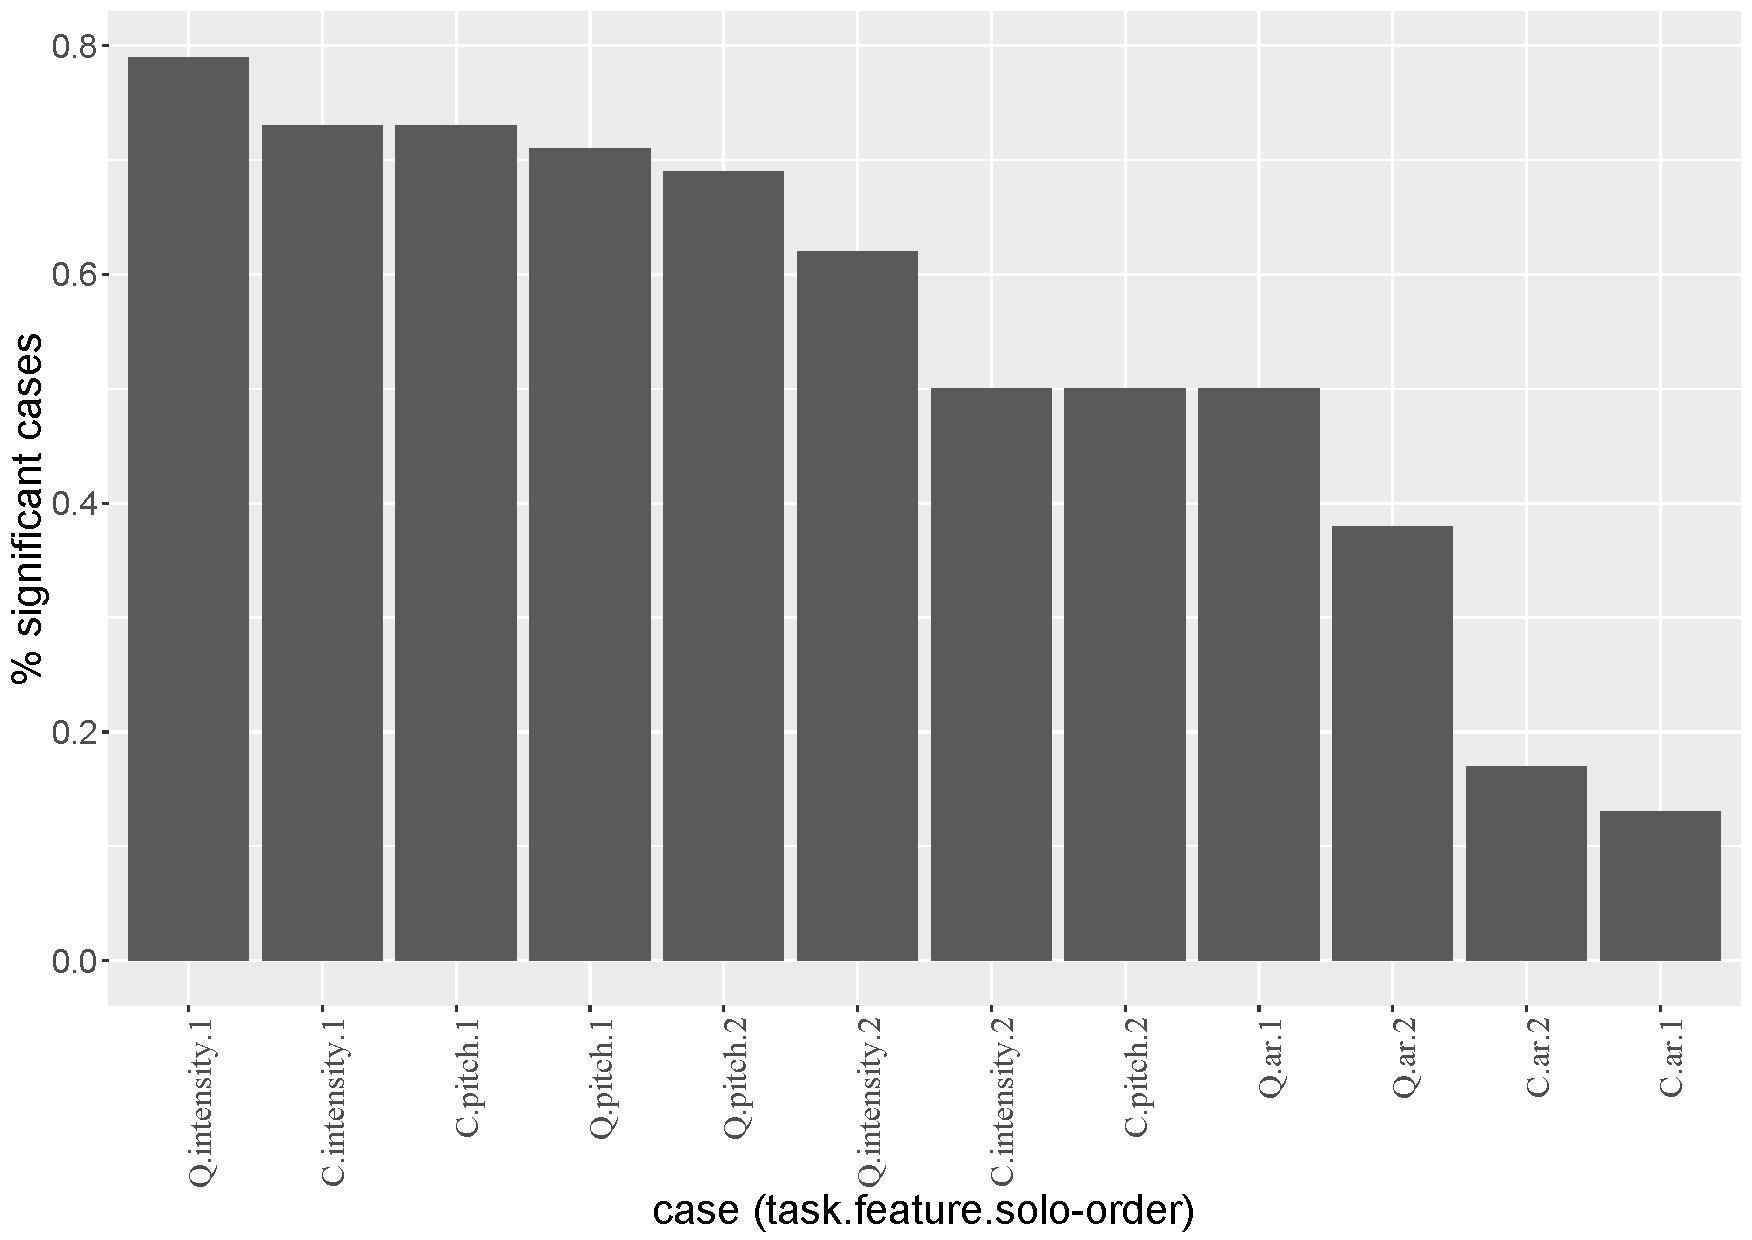
\includegraphics[width=.9\linewidth]{barplot_signif_cases}
	\caption[Per-case comparison of significant distributional differences in the crowd component]
		{Percentages of cases with a significant difference between a feature's distributions in the solo and confederate conditions.
		A case is a combination of the factors \texttt{task}, \texttt{feature}, and \texttt{order}.
		For example, the case \texttt{Q.intensity.2} contains the comparisons of intensity in interactions of the quiz task where solo condition was performed second.}
	\label{fig:signif_cases_ordered}
\end{figure}

\subsection{Temporal analysis}
\label{subsec:temporal_analysis}

Looking at the distributional differences of the target features in \ac{hds} and \ac{dds} sheds light on the general speech behaviors of the participants.
However, this analysis leaves out an important aspect of spoken interactions, namely the time dimension.
While the interaction-level distribution measures show accommodation effects based on te overall range and frequency of a feature's values, the temporal analysis adds the information as to how they changed over time.
Adding the time dimension gives an overview of an interaction's structure and reveals additional insights regarding its dynamics, such as turn lengths, turn switching, pauses, and accommodation effects.
For that, trend lines for the temporal changes needs to be calculated.
This was achieved by smoothing the measured value using \ac{loess} \citep{Cleveland1988locally}, a non-parametric regression method that deterministically fits a function to a localized subset of the data.
The fitting was done for each speaker separately over all slices of \ac{hds} and \ac{dds} with measured values of the features.
The first plot in \cref{fig:hds_dds_time} shows a case where the absolute \ac{f0} values are roughly the same in \ac{hds} and \ac{dds}, but the participant's change patterns are different.
In the \ac{dds} context, the participant generally keeps a stable distance from Alexa's voice, whereas in the \ac{hds} context the \ac{f0} values gradually get closer to the confederate's.
In both contexts, the participant's \ac{f0} starts around \SI{150}{\hertz}, but in \ac{hds} the minimum \ac{f0} is only slightly below this initial value, whereas in \ac{dds} it drops as far as \SI{25}{\hertz} lower.
A similar example is shown in the second plot in \cref{fig:hds_dds_time} for the intensity feature.
Unlike the previous example, here the absolute values between \ac{hds} and \ac{dds} steadily differ by about \SI{5}{\decibel} (matching the tendency to talk louder toward Alexa, as described above), but the overall change is similar.
That is, in both cases the intensity rises from the beginning to around a quarter of the interaction's duration, and then decreases again until the end, in \ac{hds} more quickly than in \ac{dds}, down to approximately the same value as at the beginning.
Since \cref{fig:hds_dds_time} shows two examples of the quiz task performed by two different participants, it is possible to compare the structure of these interactions as well.
As described in \cref{sec:vacc}, the quiz task in the confederate condition is designed so that the two human speakers need to find an efficient way to solve the questions using Alexa.
After improving their strategy, the lead should ultimately be taken by the participant, who interacts with Alexa to solve the questions as quickly and correctly as possible.
In both examples, the first half of the interaction contains relatively short turns and rapid addressee changes.
This might be ascribed to the fact that the participants are still trying to figure out the best way to interact with Alexa and the confederate.
Then, sometime after the middle of the interaction, there is a larger block of \ac{dds}, followed by some more turns of \ac{hds} where the participants discuss with the confederate about ways to solve the remaining questions.
Finally, the interactions end with a shorter block of \ac{dds}, in which the participants finish these last questions of the quiz.
This structure quiz task was found in most participants' performances.
%
\begin{figure}
	\vspace{-0.8cm}
	\centering
	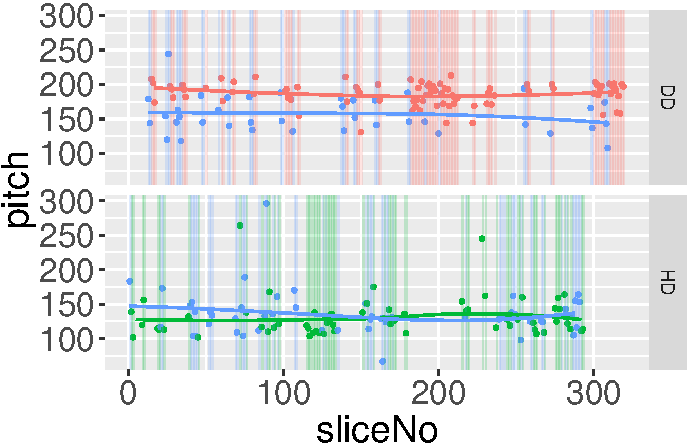
\includegraphics[width=.88\linewidth]{20171129A_Quiz_01_pitch_time_cut}
	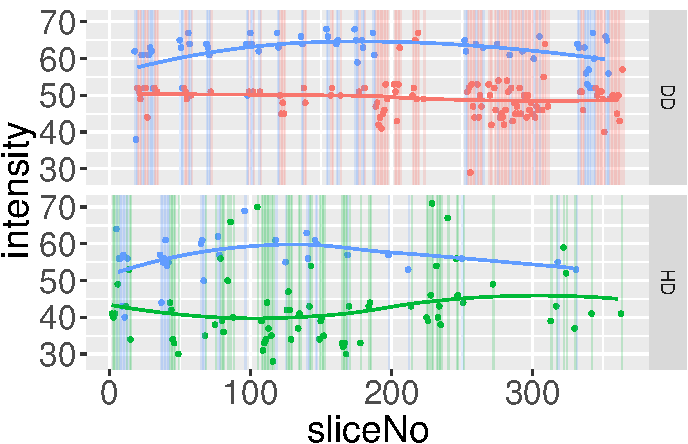
\includegraphics[width=.88\linewidth]{20171129B_Quiz_02_intensity_time_cut}
	\caption[Temporal comparison of \acs{f0} and intensity trends in \acs{hds} and \acs{dds}]
		{The changes of \acs{f0} (top; quiz task of participant 20171129A) and intensity (bottom; quiz task of participant 20171129B) over time in \ac{dds} and \ac{hds} (upper and lower parts of each plot, respectively).
		Alexa's voice is marked in red, the confederate in green, and the participant in blue.
		The timespans on the x-axis are represented by turn slices, as explained in \cref{sec:analysis_hhci}, and the y-axis shows the values of the feature.
		A slice's background color indicates the speaker in this slice and the dots with the same color show the measured value of the feature in that slice.
		The trend lines are smoothed values calculated by LOESS \citep{Cleveland1988locally}.}
	\label{fig:hds_dds_time}
\end{figure}

%Another way to look at accommodation in an interaction is in the temporal dimension.
%In this analysis, the same raw measured values were used to examine changes that occur over time.
%That is, unlike the analysis presented in \cref{subsec:distributional_analysis}, here the order of the values (i.e., their change over time) plays a major role, and effects may be found in specific time windows.
%To perform such an analysis over the entire interaction, two additional computation steps are required.
%First, each point in time must have a corresponding value for each feature produced by all speakers.

%This results in a predicted value for each slice of the conversation.
The accommodation in each conversation were further examined by measuring the contribution of the participant to the overall mutual change.
\cref{fig:condition_convergence_comparison} illustrated a comparison of a participant's changes in the solo and confederate conditions. 
The lower part of each plot shows the accommodation changes of the participant during the interaction (blue for convergence and red for divergence), and the upper part shows the floor changes.
Note that the confederate condition has fewer floor changes, because the analysis concentrates on the participant and Alexa, and the confederate turns are not shown.
The relationship between a feature's values in each slice needs to be determined to describe their temporal changes.
To investigate the accommodation effects, a measure for the relative change between slices was used, which calculates the participant's contribution to the overall change in proximity between the participant and Alexa.
Alexa's contribution is considered to be a static effect, as it is not deliberately changing its output based on the participant's speech.%, and is therefore not taken into account.
The degree of change between two slices is calculated by
%
\begin{equation}
	\label{eq:change}
	change_t = -\Delta_{t, t-1} \mid S_{part} - S_{Alexa} \mid,
\end{equation}
\eqname{Smoothed mutual change of two interlocutors}\noindent
%
where the index $t$ refers to the current slice and $S_{part}$ and $S_{Alexa}$ are the smoothed values of the participant and Alexa, respectively.
The minus sign at the front flips the value so that convergence is represented by positive values and divergence by negative values.
Subsequently, the participant's contribution toward the accommodation is calculated by
%
\begin{equation}
	\label{eq:accommodation}
	accomm(participant)_t = change_t - \Delta_{t, t-1} S_{Alexa}.
\end{equation}
\eqname{Speaker's contribution to accommodation}\noindent
%
%
\begin{figure*}[t]
	\centering
	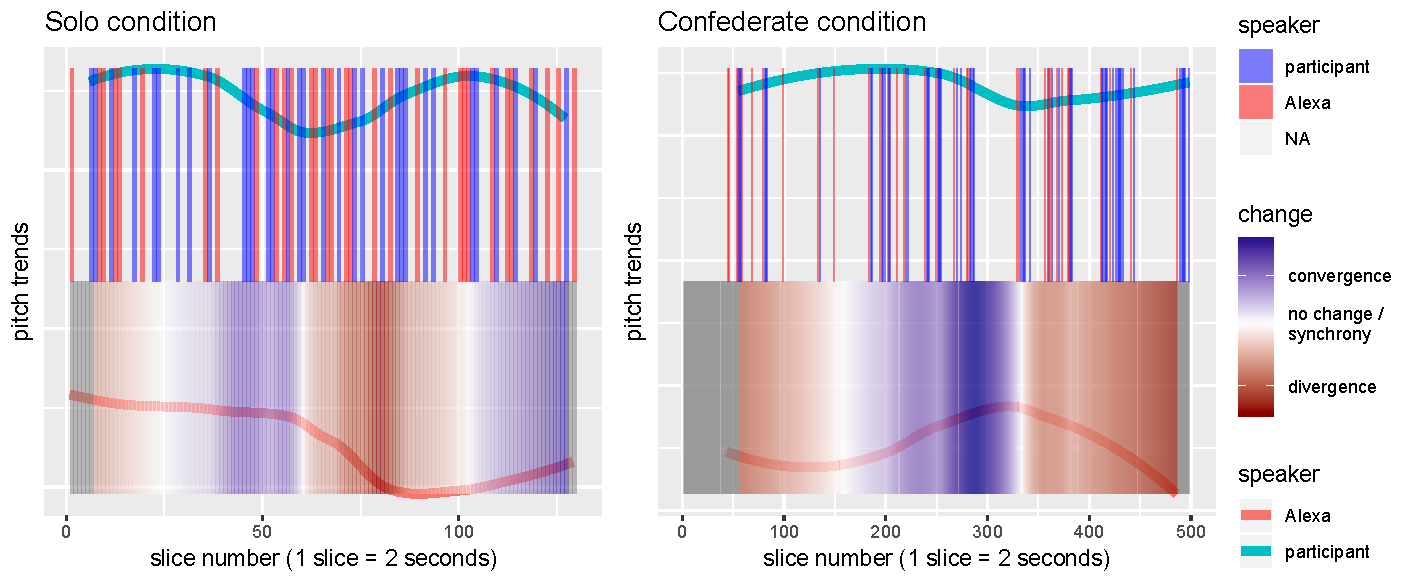
\includegraphics[width=\linewidth]{20171127B_Quiz_pitch}
	\caption[Temporal comparison of accommodation in solo and confederate conditions]
		{A comparison between \ac{f0} changes in solo (left) and confederate (right) conditions.
		The horizontal lines show the smoothed trends of the participant (blue) and Alexa (red).
		Confederate turns and omitted segments (as per \cref{subsec:annotations_hhci}), are not colored (gray).
		The vertical bars in the upper halves represent the turns of the participant (blue) and Alexa (red).
		The color-scaled vertical bars at the bottom halves show the convergence (blue) or divergence (red) level of the participant as calculated by \cref{eq:accommodation}.
		The darker the color, the greater the effect, with white indicating no change (or synchrony, in segments with both trends moving the same way).}
	\label{fig:condition_convergence_comparison}
\end{figure*}
%
The sum of the changes of each target feature produced by all participants in every interaction (i.e., a sex-task-condition-order combination) was calculated, resulting in a single value that represents the overall change per feature.
A value greater than zero means that more convergence was observed, while a negative value points to more divergence.
There were only two instances where this value was exactly zero, both for the \ac{ar} feature.
These instances were treated as cases of divergence, for their divergence spans were longer.
Using this approach, only a few interactions had no feature convergence in them, and several had all three features showing convergence.
However, a stricter threshold was applied, where a feature was considered as converging only if its overall accommodation value was higher than one standard deviation from its mean.
Based on this criterion, all interactions were categorized by the number of features that showed more convergence in them.
\Cref{fig:alluvial} summarizes this categorization for each factor.
Each line represents a single interaction, and the strata it goes through form the factor combination of this interaction.
The number of features that showed more convergence than divergence overall is marked by the color of the line.
Some tendencies emerge from this categorization:
first, in \SI{35}{\percent} of the interactions, there was at least one feature that showed convergence, but in none of them did so all three features (though there were such cases with the more tolerant criterion).
In seven interactions, two features showed convergence, two of which by male participants and five by females.
In total, males converged in \SI{5}{\percent} of all measurements and females in \SI{7}{\percent}.
Furthermore, of all converged features, \SI{58}{\percent} occurred in the solo condition, compared to \SI{42}{\percent} in the confederate condition.
However, no substantial difference between the calendar and quiz tasks was found, with \SI{49}{\percent} and \SI{51}{\percent} of the cases, respectively.
The same holds for the comparison between the two orders in which the tasks could be performed.
These results support the addition of the confederate to the interaction as the factor for less convergence occurring in interactions.
%
\begin{figure}[!t]
	\vspace{-0.5cm}
	\centering
	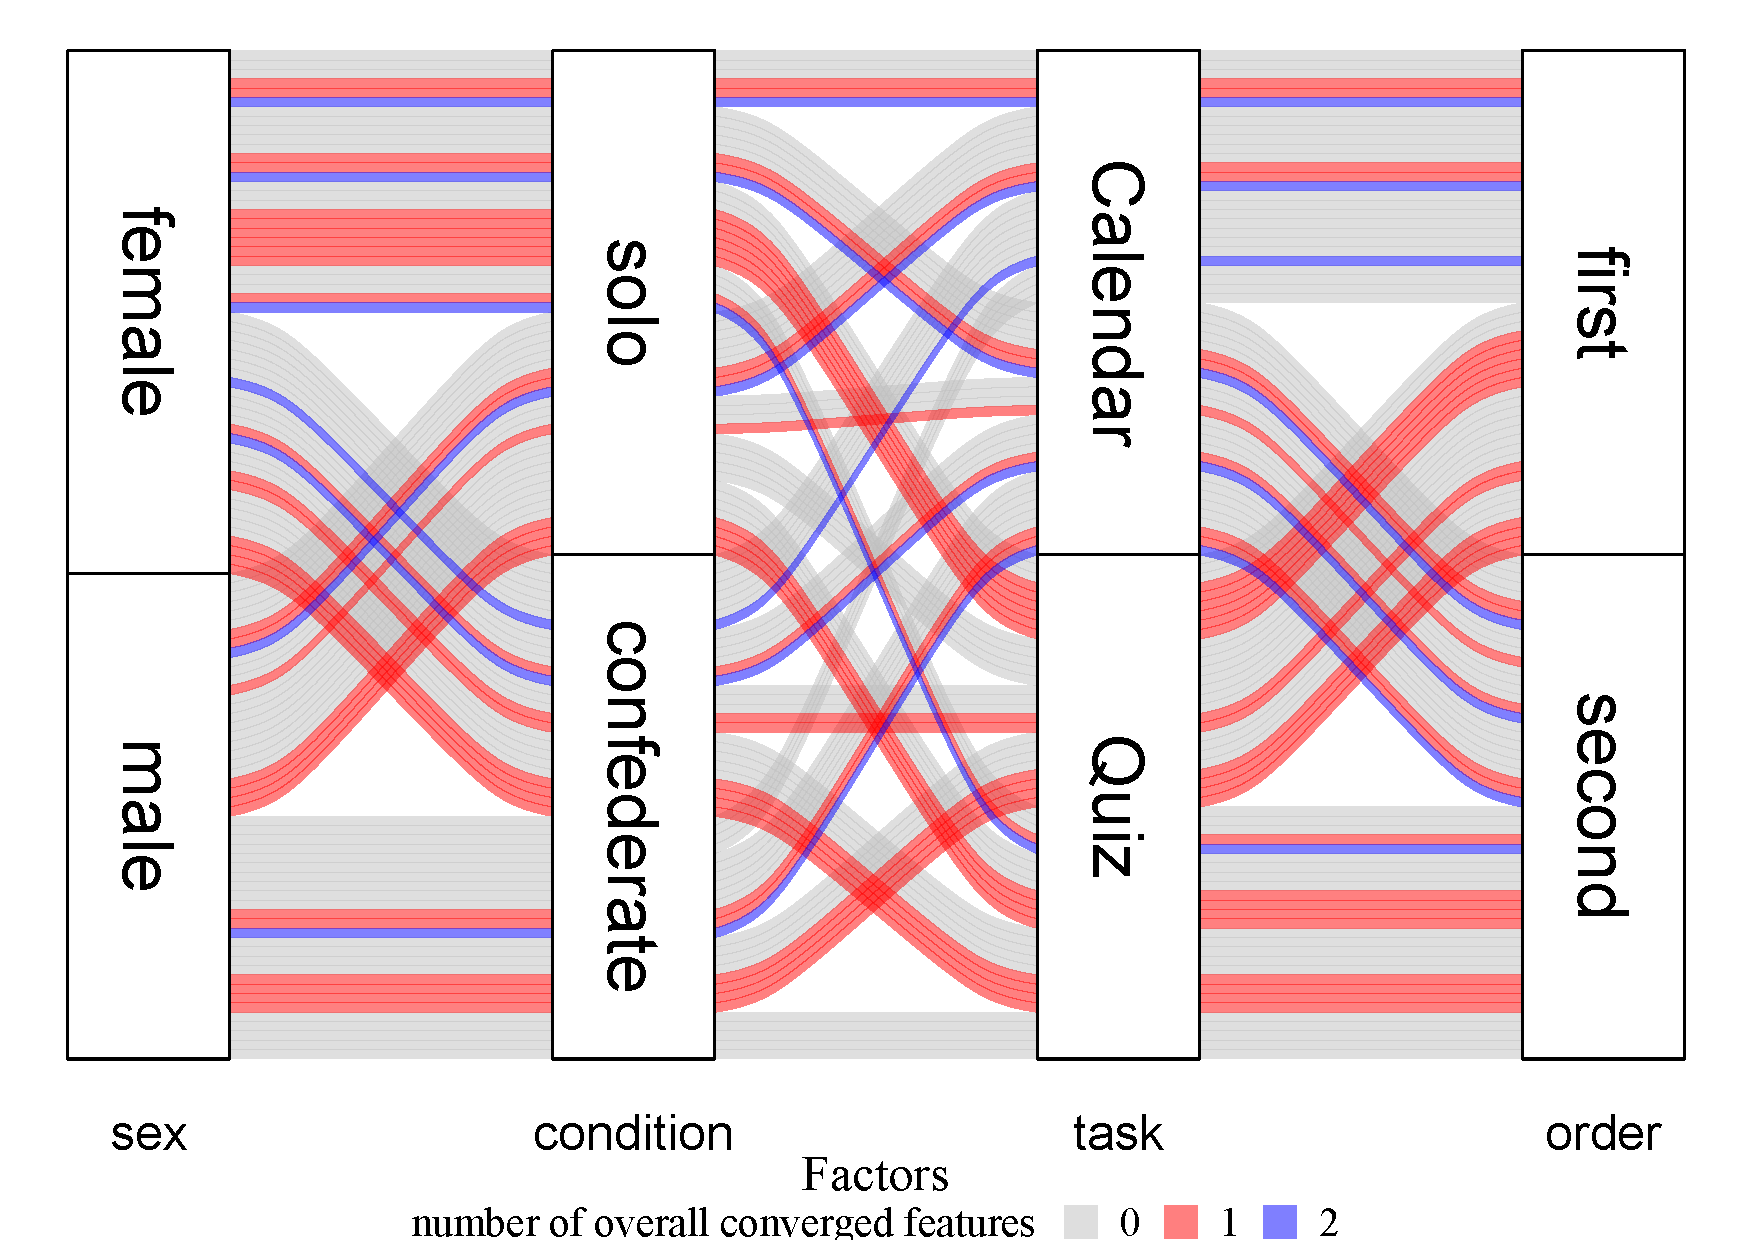
\includegraphics[width=.9\linewidth]{alluvial_4factors_numConv_strict}
	\caption[Number of features showing convergence categorized by factor]
		{Overview of the relation between the factors \texttt{sex}, \texttt{condition}, \texttt{task}, and \texttt{order} and the number of features that showed more convergence in total across all interactions.
		Each line represents one interaction.
		% The \texttt{sex} stratus refers to the sex of the participant, and the \texttt{order} stratus to the position of an interaction in the order in which the task-condition combination was performed.
		The line colors stand for the number of target features that showed overall convergence in this interaction, from none (zero features, in gray), through one (red), and up to two (blue).
		%		and up to all three features (green).
		For example, a blue line going through the strata sequence \emph{female $\rightarrow$ solo $\rightarrow$ quiz $\rightarrow$ first} represents an interaction with a female participant performing the quiz task in solo condition first, in which the participant converged in two out of the three target features.}
	\label{fig:alluvial}
\end{figure}
%
\section{Conclusion}
\label{sec:discussion_hhci}

The study in this chapter investigated vocal accommodation in \acf{hhci}.
\emph{Addressee} and \emph{crowd} components of the study examined different aspects of simulated real-world use cases, in which a human user talks alternately with a computer-based interlocutor and another human interlocutor.
The addressee component looked at differences between \acf{hds} and \acf{dds} within an interaction, while the crowd component focused on differences in \ac{dds} with and without the presence of the other human speaker.
Distributional and temporal accommodation analyses were performed in both components to provide interaction-level and time-related insights.

Three features were analyzed in the study: \acf{f0}, intensity, and \acf{ar}.
The first two features show a greater degree of difference in both components than the third.
Furthermore the changes were even greater in the crowd component, in which a human interlocutor was involved.
This indicates that not only \ac{f0} and intensity are more prone to variation than \ac{ar} in general, but also that human interlocutors trigger these variations more.
There several possible reasons for this difference.
First, computer-based agents, such as Amazon Alexa used here, do not change their speech output in any way, regardless of variations in the user's speech input.
As a social, mutual process, accommodation is more likely to be stronger if both interlocutors contribute to the overall effect.
In this study, the process can only be mutual in \ac{hds}, where another human is involved.
Nevertheless, accommodation indeed occurred in \ac{dds} as well, both with and without the presence of the confederate.
Secondly, due to this spontaneous nature of accommodation in \ac{hhi}, the participants might have automatically spoken more dynamically toward the confederate, due to the inherently expected dynamic variations is in human interlocutor.
Finally, \acp{va} (and voice-activated devices as a whole) are, in for the most part, still not performing well enough for people to speak to them as fluently and naturally as with humans.
This results in a different manner of talking to machines.
For example, users are more likely to articulate whole sentences, typically without reformulating, when requested to repeat their utterance by the device, whereas human interlocutors are capable of requesting and conveying corrections with shorter segments using intonation and other means.
Furthermore, although generally more seldom vary, users tend to reduce their \ac{ar} when repeating their utterances to the device, or when trying to be more clear.
This resembles the way people talk to children when they want to be more clear.
However, due to the way \ac{asr} systems are trained, more often than not this achieves the opposite result.
While participant did not change their \ac{ar} much toward Alexa, they did show accommodation in \ac{f0}.
This can be explained by the natural difference in male and female \ac{f0} ranges, which leaves room for accommodation for participants of both sexes (Alexa used a female voice while the confederate was always male).
In that case, the results shown here point to the fact that the participants generally treated Alexa as a human interlocutor with regards to \ac{f0} behavior, as opposed to talking to Alexa using a more monotonous \ac{f0}.
This happened despite Alexa not varying her \ac{f0} beyond the sentence-level intonation.
A similar effect was found for intensity.
Since the device and the confederate were squally distanced from the participants, there was no apparent reason for the participants to speak more loudly with either interlocutor.
Therefore, an explanation of the tendency to speak more loudly to the device may come from the intuition that a computer-based system has a harder time understanding human speech and therefore needs a clearer signal (also using lower \ac{ar}, as explained above).
This stands in line with the interpretation that humans sometimes treat voice-activated devices as humans who need a hyper-articulated speech signal to understand, like toddlers or language learners\footnote{In a sense, this analogy is correct, as the devices -- or rather their \ac{asr} components -- indeed learn to process speech signals.
Despite that, this process is different than the way babies acquire spoken language, and therefore such projection on the speech style does not help the device improving its understanding of the user.
Moreover, slower or disfluent speech may actually hinder the systems' understanding, as they are typically not trained on this kind of speech.}.
Another explanation may be the illusion that Alexa feels more distant than the human interlocutor because she is not an embodied agent \citep[cf.][and see \cref{sec:types_of_sdss} for further details]{Staum2010virtually, Gijssels2016speech}.
Keeping in mind that humans strive to communicate as efficiently as possible, it seems like changing these features helped the participants -- or at least felt like they did -- to interact better with Alexa.
Regardless of whether this roots from the unconscious attempt to treat the device as a social actor in the conversation \citep{Nass1994computers, Nass2000machines} or the fact that accommodation occurs, even if to a lesser extent, even when it's not mutual, the effect still took place.
This is, however, not the case with \ac{ar}, which shows a lower percentage of significant differences.
This indicates that \ac{ar} does not tend to vary as much as \ac{f0} and intensity, which stands in line with other studies, like \citet{Schweitzer2013convergence}.
Slower, more carefully articulated speech, occurs less often in regular speech than louder speech or higher pitch.
Such enhanced articulation not only takes longer to produce, but also requires more effort, making it a less preferred way to communicate, unless necessary.
In this somewhat formal experimental setting, participants are likely to speak more slowly than usual, and the motivation to complete the task in a short time encourages them not to speak even more slowly.
This supports the hypothesis that extra slow speech would only be used when necessary, e.g., when a repetition is required due to a recognition error on the system's side.
Once the misunderstanding was resolved, participants' went back to their original \ac{ar}.
These local changes may suggest that changes in \ac{ar} are done more consciously than in other phonetic features.

The results presented in \cref{tab:results_hhci_addressee,tab:signif_conditions} show that for all three features
\begin{enumerate*}[(a)]
	\item the distributions differed more when the participants first interacted with the device alone, and
	\item more convergence was aggregated in the task that was performed first.
\end{enumerate*}
This demonstrates the influences of the \texttt{order} factor.
Furthermore, the factors \texttt{sex} and \texttt{task} indicate that female participants showed a slightly higher amount of convergence in total than male participants, and that the performed task did not play role the increase or decrease of convergence.
The first speech input a participant encounters may cause a priming effect that, together with the natural tendency to converge to an interlocutor, results in a greater change in interactions that occur first.
However, the interchangeability of input (here, both \ac{hhi} and \ac{hci}) seems to hinder the ability of the participants to converge to Alexa.
One explanation for this may be that it is more natural for humans to accommodate to other humans, so once another human is involved, the accommodation towards the computer-based interlocutor is annulled.
Another possible explanation is that due to the multiple interlocutors, the participants do not have a steady target to accommodate toward, which leads to a weakened convergence effect.
This is confirmed by the higher number of convergence instances in the solo condition compared to the confederate condition in both the temporal and distributional analyses.
This could be explained as a reaction to a more stable vocal target (especially since Alexa generally doesn't change her voice much) than when alternating between two interlocutors.
Since \ac{hci} still lacks the mutuality of accommodation effects, the question arises whether these tendencies would be stronger in interactions with a single human versus interactions with two human speakers simultaneously.
The higher number of convergence instances by female participants may be ascribed to the \ac{va} using a voice of the same sex and could be further investigated by using a \ac{va} with a male voice.

%In conclusion, it is clear that accommodation effects and tendencies were present in both conditions, which is reassuring for future multiparty \ac{hci} accommodation research.
%Two main open questions remain concerning the temporal aspect of interactions.
%The first has do to with analysis on the speech \emph{signal level}, where the changes in measures over time can capture phenomena like convergence or divergence.
%In a more comprehensive analysis in this direction, more detailed patterns may emerge.
%Such an analysis can concentrate on one context or on comparing patterns in both \ac{hds} and \ac{dds}.
%Additionally, more features can be measured to reveal more details regarding speech behavior.
%The second may highlight behavioral patterns of the conversation on the \emph{turn levels}.
%This can include a closer examination of the interaction structure as a whole, the dynamics of turn changes, pauses and repetitions, etc.
%Such an analysis can be performed on interactions in solo and confederate condition to inspect whether humans deal with the same task performed with a computer alone differently than when another human is involved.